% !TEX root = ./Basilisk-MRP_PD-2019-03-29.tex


\begin{figure}[h]
	\centerline{
		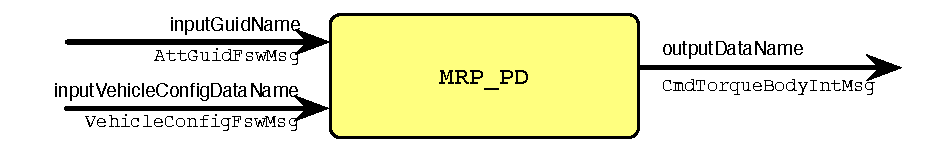
\includegraphics{Figures/moduleImg}
	}
	\caption{Illustration of the module input and output messages.}
	\label{fig:moduleImg}
\end{figure}


\section{Model Description}
This attitude feedback module using the MRP feedback control related to the control in section 8.4.1 in Schaub and Junkins.\cite{schaub}
\begin{equation}
			\label{eq:Lr}
			\bm L_{r} =  -K \bm\sigma - [P] \delta\bm\omega   + [I](\dot{\bm\omega}_{r} - [\tilde{\bm\omega}]\bm\omega_{r}) 
			+[\tilde{\bm \omega}_{r}] ]
			[I]\bm\omega   - \bm L
\end{equation}

Note that this control solution creates an external control torque which must be produced with a cluster of thrusters.  No reaction wheel information is used here.  Further, the feedback control component is a simple proportional and derivative feedback formulation.  As shown in Reference~\citenum{schaub}, this control can asymptotically track a general reference trajectory given by the reference frame $\cal R$.  





